%-------------------------------------------------------------------------------
%	CAPITOLO 36
%-------------------------------------------------------------------------------

\chapter{L'atto di divisione tra cognati}
Il notaio \index[Personaggi]{Pirazzoli (notaio)}Pirazzoli si era seduto, lo scrivano \index[Personaggi]{Peppino (scrivano)}Peppino aveva steso la carta bollata sul tavolo, tre cognati e due consorti siedevano intorno al tavolo. \\
\indent Un cognato: <<Alora te t'am dé zeczent frenc...\footnote{<<Allora te mi dai cinquecento lire>>}>>\\
\indent Il secondo cognato: <<No ad deg sol zent scud...>>\footnote{<<No ti dò solo cento scudi>>}\\
\indent Il primo cognato: <<L'è pù l'istes.\footnote{<<È lo stesso" infatti 1 scudo equivaleva a 5 lire}>>\\
\indent Il secondo cognato: <<No a ti darò me e zeczent frenc...\footnote{<<Te li dò io le cinquecento lire...>>}>> tira fuori un lungo stile e si avventa sul primo cognato, che infila la porta e fugge a gambe levate inseguito...\\
\indent Terzo cognato e sorelle: <<Un spò scorrar cun cucalà\footnote{<<Non si può parlare con quello là>>}>>\\
\indent Notaio: <<Me ne vado anch'io finché la strada è libera e buona...>>\\
\index[Personaggi]{Peppino (scrivano)}Peppino, raccolse la carta e l'infilò nella cartella e via... dietro al notaio.\\

\indent Un'altra volta il primo cognato, sempre per questione di somme nelle quali era profondo, aveva disteso, in piazza su di una panca, certi lavori.\\
\indent Un cliente: <<Ti dò una lira e mezzo>>\\
\indent Primo cognato: <<No, a voi trenta bulè\footnote{<<No voglio trenta soldi>> - 1 soldo era equivalente a 5 centesimi di lira, quindi 30 soldi erano esattamente 1 lira e mezzo}>>\\
\indent Cliente: <<T'si mat...\footnote{<<Sei matto...>>}>>\\
\indent Primo cognato credendosi preso in giro: <<A ti darò me la lira e mezzo...\footnote{<<Te la darò io la lira e mezzo...>>}>> e gli si avventò per picchiarlo.\\
\indent È da sperare che questo bravo primo cognato non venga mandato dai sindacati, per turno di lavoro, a prestare la sua opera alla commissione dei cambi con l'estero.\\

\vspace{1cm}
\centerline{\rule{1.5cm}{0.4pt}}
\vspace{1cm}

 \begin{figure}[htb]
    \centering
    %\vspace{-0.7cm}
    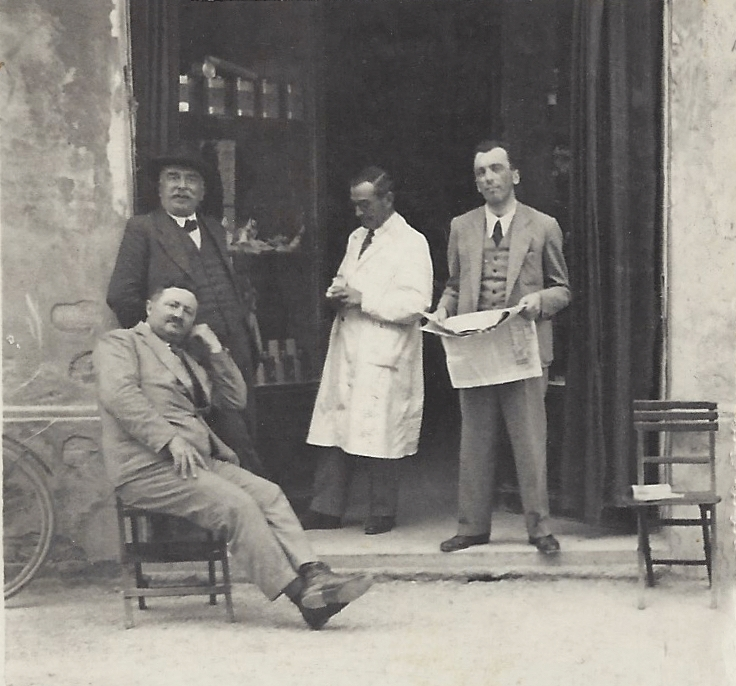
\includegraphics[width=\textwidth]{farmaciamingazzi}
    \caption[Entrata Farmacia con Mingazzi]{L'entrata della farmacia comunale  \index[Luoghi]{Farmacia Comunale} in via Mazzini. Nando \index[Personaggi]{Isani Nando}Isani in camice bianco. Seduto Stefano \index[Personaggi]{Mingazzi Stefano}Mingazzi, dietro il dott. Cassiano \index[Personaggi]{Meruzzi dott. Cassiano}Meruzzi. In piedi col giornale il direttore del Credito Romagnolo Pasi.
	\label{fig:farmaciamingazzi}}
    %\vspace{-0.3cm}
\end{figure}